\documentclass{article}
\usepackage[utf8]{inputenc}
\usepackage[spanish]{babel}
\usepackage{listings}
\usepackage{subfigure}
\usepackage{graphicx}
\usepackage{url}
\usepackage{multirow}
\usepackage{color}
\usepackage{booktabs}


\setlength{\parindent}{0pt}
\setlength{\parskip}{1em}


\definecolor{mygreen}{rgb}{0,0.6,0}
\definecolor{mygray}{rgb}{0.5,0.5,0.5}
\definecolor{mymauve}{rgb}{0.58,0,0.82}
\lstset{ 
  backgroundcolor=\color{white},   % choose the background color; you must add \usepackage{color} or \usepackage{xcolor}; should come as last argument
  basicstyle=\footnotesize,        % the size of the fonts that are used for the code
  breakatwhitespace=false,         % sets if automatic breaks should only happen at whitespace
  breaklines=true,                 % sets automatic line breaking
  captionpos=b,                    % sets the caption-position to bottom
  commentstyle=\color{mygreen},    % comment style
  deletekeywords={...},            % if you want to delete keywords from the given language
  escapeinside={\%}{)},          % if you want to add LaTeX within your code
  extendedchars=true,              % lets you use non-ASCII characters; for 8-bits encodings only, does not work with UTF-8
  firstnumber=1,                % start line enumeration with line 1000
  frame=single,	                   % adds a frame around the code
  keepspaces=true,                 % keeps spaces in text, useful for keeping indentation of code (possibly needs columns=flexible)
  keywordstyle=\color{blue},       % keyword style
  language=Octave,                 % the language of the code
  morekeywords={*,...},            % if you want to add more keywords to the set
  numbers=left,                    % where to put the line-numbers; possible values are (none, left, right)
  numbersep=5pt,                   % how far the line-numbers are from the code
  numberstyle=\tiny\color{mygray}, % the style that is used for the line-numbers
  rulecolor=\color{black},         % if not set, the frame-color may be changed on line-breaks within not-black text (e.g. comments (green here))
  showspaces=false,                % show spaces everywhere adding particular underscores; it overrides 'showstringspaces'
  showstringspaces=false,          % underline spaces within strings only
  showtabs=false,                  % show tabs within strings adding particular underscores
  stepnumber=1,                    % the step between two line-numbers. If it's 1, each line will be numbered
  stringstyle=\color{mymauve},     % string literal style
  tabsize=2,	                   % sets default tabsize to 2 spaces
  title=\lstname                  % show the filename of files included with \lstinputlisting; also try caption instead of title
}
\title{Tarea 4}

\author{5271}
\date{\today}

\begin{document}
\maketitle

\section{Algoritmos generadores de grafos.}

Gracias a la versatilidad de Los grafos como modelo de representación de datos, los procesos aleatorios de generación de grafos también son relevantes en aplicaciones que van desde la física, biología a la sociología \cite{Nobari} .

Para realizar la tarea se seleccionaron tres algoritmos generadores de grafos de la biblioteca de networkx, con el objetivo de crear los grafos con pesos con distribución normal (como se muestra en la figura \ref{fig1 }de la página \pageref{fig1}) a los que se le aplicaran los algoritmos de flujo máximo para realizar los experimentos requeridos. Los tres algoritmos escogidos son de generación aleatorias.
 
Los algoritmos escogidos fueron los siguientes:

\begin{itemize}
  \item\textit{Erdos renyi graph} (en el modelo \textit {G (n, p)}, el grafo se construye conectando los \textit{n} vértices al azar. Cada arista se incluye en el grafo con probabilidad \textit{p} independiente de cualquier otro borde)  \cite{erg}.  
   \item\textit{Fast gnp random graph} (este algoritmo recibe como parámetros \textit{n} números de vértices y probabilidad \textit{p} de ocurrencia de aristas, el mismo devuelve un grafo aleatorio) \cite{rgf}.
	\item\textit{Binomial graph} (este algoritmo recibe como parámetros \textit{n} números de vértices y probabilidad \textit{p} de ocurrencia de aristas, el mismo devuelve un grafo aleatorio, para grafos dispersos (para valores pequeños de \textit{p}), \textit{Fast gnp random graph} es un algoritmo más rápido) \cite{bg}.
	
En la figura \ref{fig2} de la \pageref{fig2} se muestra ejemplos de grafos generados por los algoritmos antes mencionados.
\end{itemize}
\begin{center}
\begin{figure}[h]
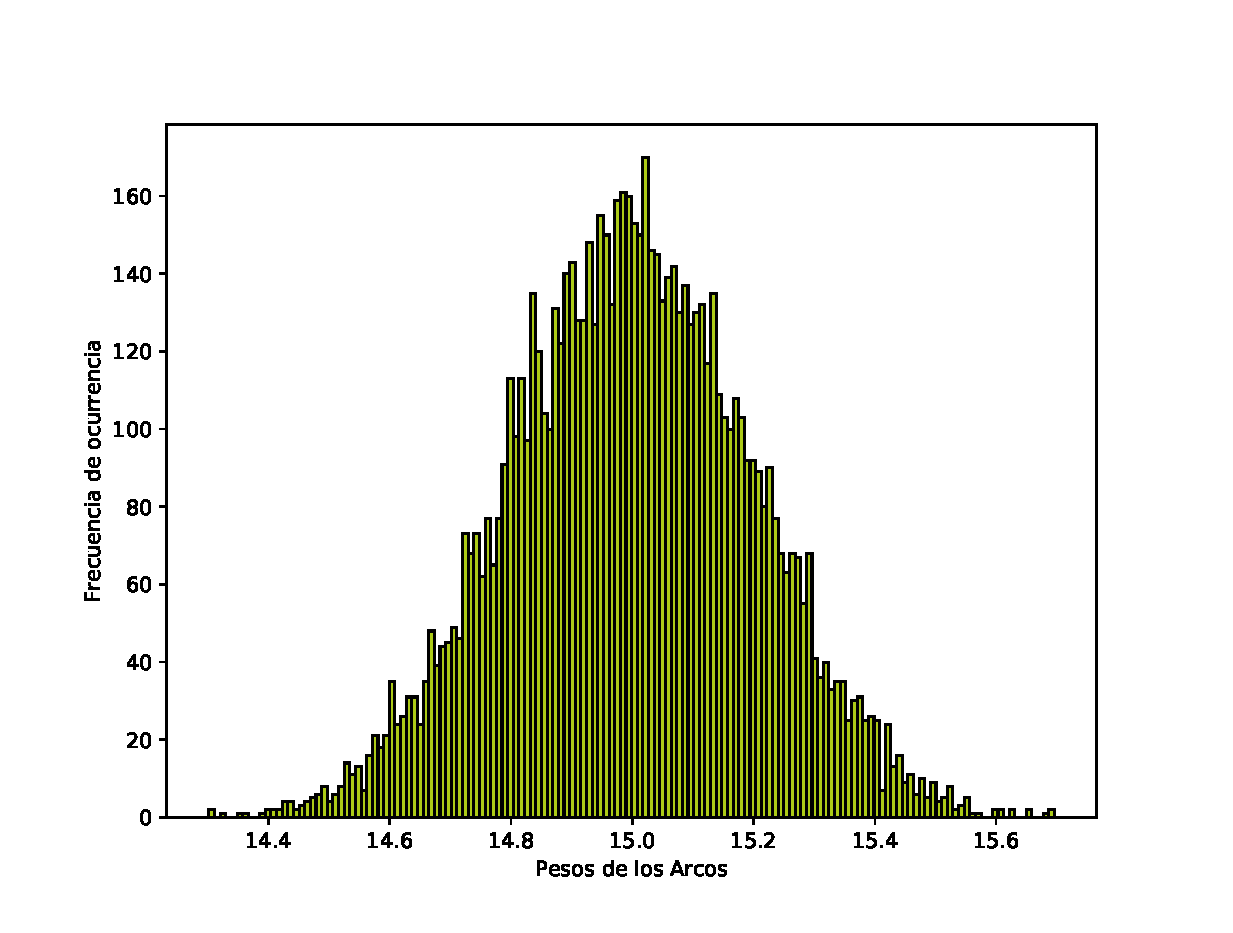
\includegraphics[scale=0.7]{histograf.eps}
\caption{Histograma de distribución de los pesos.}
\label{fig1}
\end{figure}
\end{center}
\begin{figure}[h]

\subfigure[\textit{Binomial graph}, con 30 vértices]{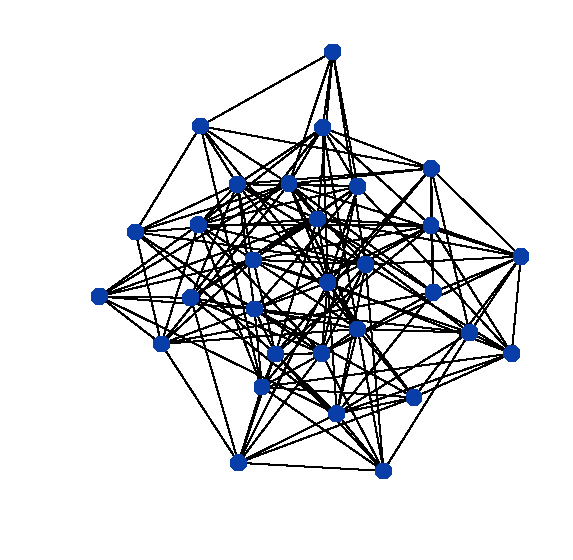
\includegraphics[scale=0.5]{binomialgraph.eps}}
\subfigure[\textit{Erdos renyi graph}, con 20 vértices]{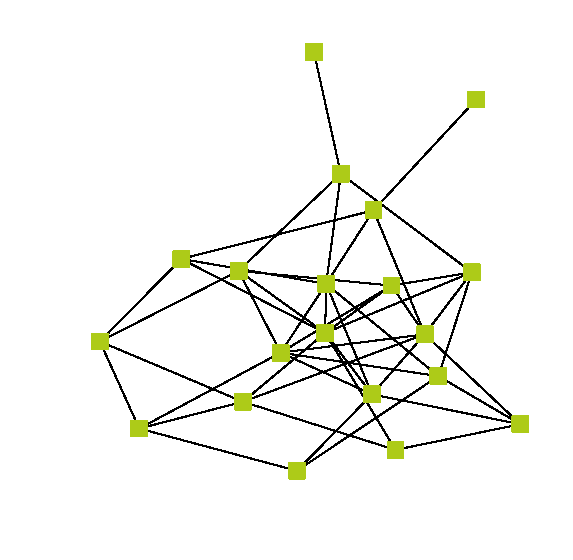
\includegraphics[scale=0.5]{erdosrenyigraph.eps}}
\subfigure[\textit{Fast gnp random graph}, con 15 vértices]{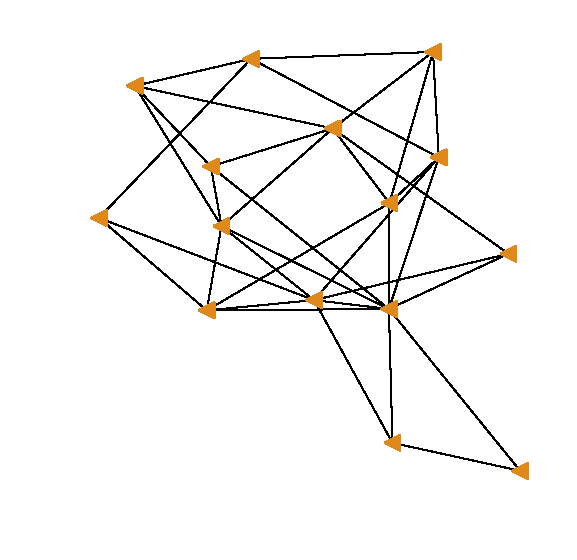
\includegraphics[scale=0.5]{fastgnprandomgraph.eps}}

\caption{Ejemplo de grafos generados con los algoritmos seleccionados.}
\label{fig2} 
\end{figure}


\newpage
\section{Algoritmos de flujo máximo.}
En los problemas de flujo en redes, las aristas representan vías por las que puede circular elementos: datos, agua, corriente eléctrica, entre otras. Los pesos de las aristas representan la capacidad máxima de una vía: velocidad de una conexión, volumen máximo de agua, voltaje de una línea eléctrica, entre otras; aunque es posible que la cantidad real de flujo sea menor.
 
El problema del flujo máximo consiste en lo siguiente: dado un grafo con pesos, $G = (V, A, W)$, que representa las capacidades máximas de los canales, un vértice fuente $f$ y otro sumidero $s$ en $ V $, encontrar la cantidad máxima de flujo que puede circular desde $f$ hasta $s$.

En la librería de networkx encontramos varios algoritmos con los que podemos atacar los problemas de flujo máximo, para la realización de esta tarea se escogerán tres algoritmos de dicha librería.

Los algoritmos escogidos fueron los siguientes:
\begin{itemize}
  \item\textit{Shortest augmenting path} (es uno de los enfoques más clásicos para la máxima coincidencia y los problemas de flujo máximo. Sorprendentemente, aunque esta idea es una de las técnicas más básicas, está lejos de ser completamente entendida. Es más fácil hablar de ello introduciendo el problema de emparejamiento bipartito en línea \cite{Bosek2018}. Este algoritmo encuentra el flujo máximo de un solo producto utilizando la ruta de aumento más corto y devuelve la red residual resultante después de calcular el flujo máximo).   
   \item\textit{maximum flow} (Encuentra la ruta por la cual pasa la máxima cantidad de flujo, recibe como parámetros un grafo $G$, una fuente $f$, un sumidero $s$ y además una capacidad que de no tenerla, se considera que el borde tiene una capacidad infinita. Se puede aplicar en grafos tanto dirigidos como no dirigidos.) \cite{mf}.
	\item\textit{Preflow push} (encuentra un flujo máximo de un solo producto utilizando el algoritmo de empuje previo al flujo de la etiqueta más alta. Esta función devuelve la red residual resultante después de calcular el flujo máximo. Este algoritmo tiene un tiempo de ejecución de $ O(n^{2}\sqrt{m})$ para $n$ vértices y $m$ aristas.) \cite{gc}.
\end{itemize}
\section{Generación de datos.}
Con el objetivo de realizar las mediciones de los tiempos de ejecución de los algoritmos de flujo máximo seleccionados se desarrolló el siguiente código.

En primer lugar, se crea una función ($Algoritmo_FM()$) que recibe como parámetros el algoritmo de flujo máximo ($algoritmoF$) que se va a utilizar, el grafo al que se le aplicara el algoritmo ($Graf$), la fuente ($fuente$) y sumidero ($sumidero$). Al llamar esta función se genera con cada ejecución los datos que son guardados en un \textit{data frame} del cual se muestra un fragmentó en el cuadro \ref{tab:addlabel} de la página \pageref{tab:addlabel}.

\begin{center}
\lstinputlisting[language=Python, firstline=13, lastline=35]{Generar_datos.py}
\end{center}


% Table generated by Excel2LaTeX from sheet 'Hoja1'
\begin{center}

\begin{table}[htbp]
  \centering
  \caption{Fracmento de \textit{data frame} generado. }
  \resizebox{\textwidth}{!}{
    \begin{tabular}{lllrrrrrrrr}
    \toprule
    \textbf{grafo} & \textbf{generador} & \textbf{algoritmo\_fm} & \multicolumn{1}{l}{\textbf{vertices}} & \multicolumn{1}{l}{\textbf{densidad}} & \multicolumn{1}{l}{\textbf{aristas}} & \multicolumn{1}{l}{\textbf{f}} & \multicolumn{1}{l}{\textbf{s}} & \multicolumn{1}{l}{\textbf{mediana}} & \multicolumn{1}{l}{\textbf{varianza}} & \multicolumn{1}{l}{\textbf{desv}} \\
    \midrule
    v256a8140 & fast\_gnp & shortest\_a\_path & 256   & 0.24939 & 8140  & 33    & 101   & 0.06247 & 0.00004 & 0.00618 \\
    v256a8141 & fast\_gnp & edmonds\_karp & 256   & 0.24939 & 8140  & 33    & 101   & 0.04692 & 0.00001 & 0.00318 \\
    v256a8142 & fast\_gnp & preflow\_push & 256   & 0.24939 & 8140  & 33    & 101   & 0.08225 & 0.00025 & 0.01596 \\
    v256a8143 & fast\_gnp & shortest\_a\_path & 256   & 0.24939 & 8140  & 33    & 101   & 0.06251 & 0.00004 & 0.00638 \\
    v256a8144 & fast\_gnp & edmonds\_karp & 256   & 0.24939 & 8140  & 33    & 101   & 0.05291 & 0.00007 & 0.00834 \\
    v256a8145 & fast\_gnp & preflow\_push & 256   & 0.24939 & 8140  & 33    & 101   & 0.08253 & 0.00017 & 0.01296 \\
    v256a8146 & fast\_gnp & shortest\_a\_path & 256   & 0.24939 & 8140  & 33    & 101   & 0.06903 & 0.00020 & 0.01398 \\
    v256a8147 & fast\_gnp & edmonds\_karp & 256   & 0.24939 & 8140  & 33    & 101   & 0.05296 & 0.00003 & 0.00566 \\
    \bottomrule
    \end{tabular}%
    }
  \label{tab:addlabel}%
\end{table}%
\end{center}
En este otro fragmentó del código es donde se generan los grafos y se llama la función ($Algoritmo_FM()$).
\begin{center}
\lstinputlisting[language=Python, firstline=38, lastline=100]{Generar_datos.py}
\end{center}


\section{Resultados del Análisis de los datos.}

Con los datos recopilado de las ejecuciones de los tres algoritmos de flujo máximo con los ciento veinte grafos y sus cinco combinaciones de fuentes y sumidero, se realizó una serie de diagramas y pruebas estadísticas. A continuación, se muestra un el fragmento de código donde se lleva a cabo lo antes mencionado.

 
\begin{center}
\lstinputlisting[language=Python, firstline=12, lastline=62]{Analisis_datos.py}
\end{center}
\subsection{Análisis de varianza (ANOVA).}
El análisis de varianza (ANOVA) es la técnica central en el análisis de datos experimentales. La idea general de esta técnica es separar la variación total en las partes con las que contribuye cada fuente de variación en el experimento. En el caso de los diseños completamente al azar se separan la variabilidad debida a los tratamientos y la debida al error. Cuando la primera predomina sobre la segunda, es cuando se concluye que las medias son diferentes. Cuando los tratamientos no dominan contribuyen igual o menos que el error, por lo que se concluye que las medias son iguales \cite{ade}.

Para analizar si los diferentes factores (algoritmo generador de grafo, algoritmo de flujo máximo, numero de vértices y densidad del grafo) influían en la variable dependiente \textit{tiempo de ejecución} se realizó un ANOVA de un factor para cada caso. 

\subsubsection{Influencia del algoritmo generador de grafos en el tiempo de ejecución.}
El siguiente cuadro muestra el resultado de la aplicación del ANOVA.



\begin{table}[htbp]
  \centering
  \caption{ANOVA, relación del algoritmo generador con el \textit{tiempo de ejecución}}
    \begin{tabular}{lrrrlll}
    \toprule
    \textbf{Factor} & \multicolumn{1}{l}{\textbf{SS}} & \multicolumn{1}{l}{\textbf{DF}} & \multicolumn{1}{l}{\textbf{MS}} & \textbf{F} & \textbf{p-unc} & \textbf{np2} \\
    \midrule
    generador\_grafo & 0.280 & 2     & 0.140 & \multicolumn{1}{r}{0.354} & \multicolumn{1}{r}{0.702} & \multicolumn{1}{r}{0} \\
    \textit{Within} & 712.085 & 1797  & 0.396 & -     & -     & - \\
    \bottomrule
    \end{tabular}%
  \label{tab:t2}%
\end{table}%
En el cuadro \ref{tab:t2} se muestra que no existen diferencia entre las medianas de los grupos de factores ya que el $p-unc$ es mayor que $0.05$ por lo que se acepta la hipótesis de que el tipo de generador no influye en el \textit{tiempo de ejecución}. Esto se puede observar en la figura \ref{fig4} de la página \pageref{fig4}. 

\newpage
\begin{center}
\begin{figure}[htbp]
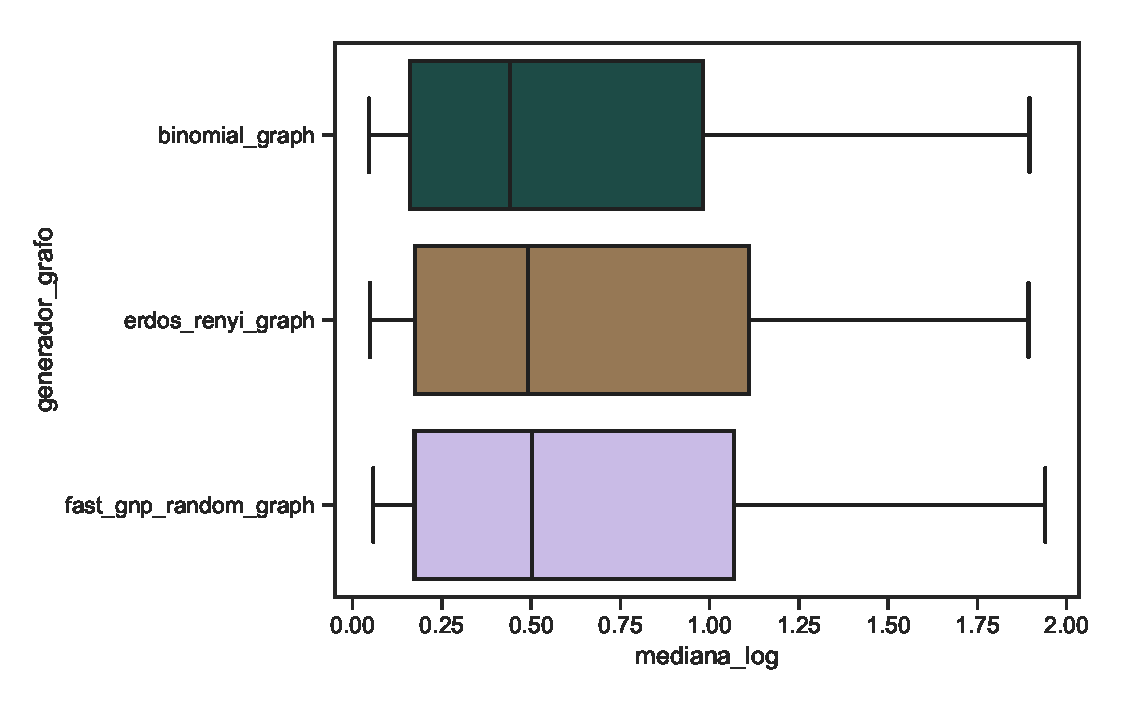
\includegraphics[scale=0.6]{boxplotgeneradorgrafo.eps}
\caption{Diagrama de caja y bigotes que relaciona los tiempos de ejecución con los algoritmos generadores de grafos.}
\label{fig4}
\end{figure}
\end{center}
\subsubsection{Influencia del algoritmo de flujo máximo en el tiempo de ejecución.}
El siguiente cuadro muestra el resultado de la aplicación del ANOVA.

% Table generated by Excel2LaTeX from sheet 'ANOVAalgoritmo_fm'
\begin{table}[htbp]
  \centering
  \caption{ANOVA, relación del algoritmo de flujo máximo con el \textit{tiempo de ejecución}}
    \begin{tabular}{lrrrlll}
    \toprule
    \textbf{Factor} & \multicolumn{1}{l}{\textbf{SS}} & \multicolumn{1}{l}{\textbf{DF}} & \multicolumn{1}{l}{\textbf{MS}} & \textbf{F} & \textbf{p-unc} & \textbf{np2} \\
    \midrule
    algoritmo\_fm & 1.499 & 2     & 0.749 & \multicolumn{1}{r}{1.895} & \multicolumn{1}{r}{0.151} & \multicolumn{1}{r}{0.002} \\
    \textit{Within} & 710.867 & 1797  & 0.396 & -     & -     & - \\
    \bottomrule
    \end{tabular}%
  \label{tab:t3}%
\end{table}%
En el cuadro \ref{tab:t3} se muestra que no existen diferencia entre las medianas de los grupos de factores ya que el $p-unc$ es mayor que $0.05$ por lo que se acepta la hipótesis de que el tipo de algoritmo no influye en el \textit{tiempo de ejecución}. Esto se puede observar en la figura \ref{fig5} de la página \pageref{fig5}. 
\begin{center}
\begin{figure}[htbp]
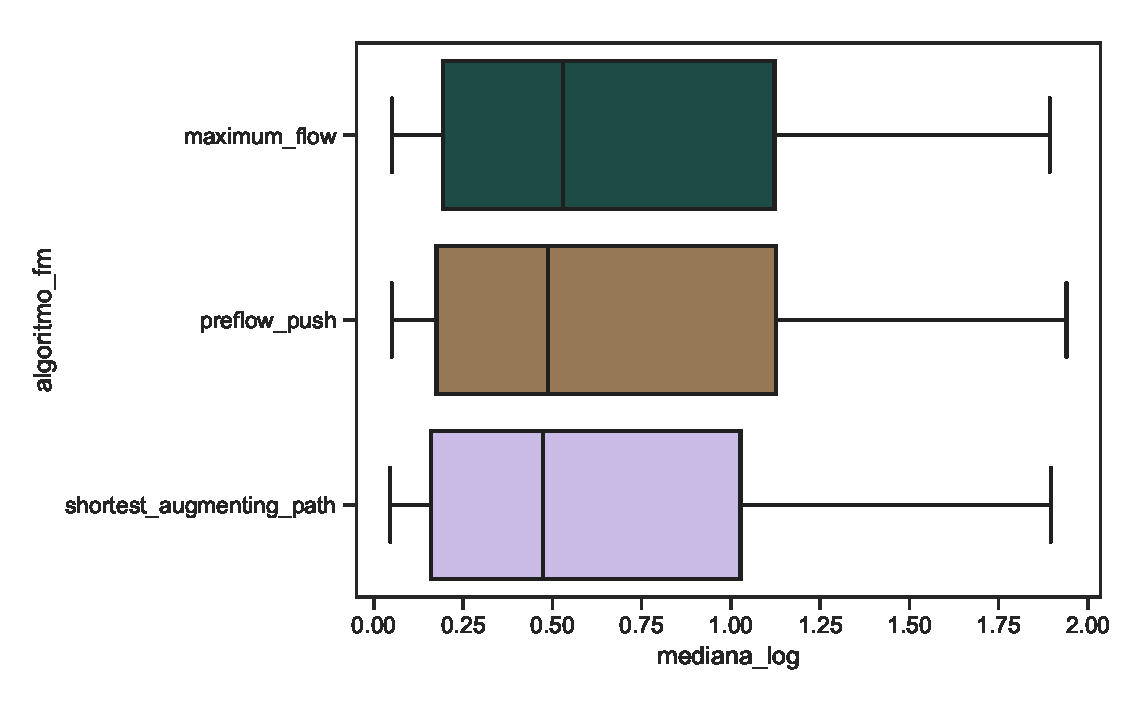
\includegraphics[scale=0.6]{boxplotalgoritmofm.eps}
\caption{Diagrama de caja y bigotes que relaciona los tiempos de ejecución con los algoritmos de flujo máximo.}
\label{fig5}
\end{figure}
\end{center}
\newpage

\subsubsection{Influencia del número de vértices en el tiempo de ejecución.}
El siguiente cuadro muestra el resultado de la aplicación del ANOVA.

% Table generated by Excel2LaTeX from sheet 'ANOVAvertices'
\begin{table}[htbp]
  \centering
  \caption{ANOVA, relación del número de vértices con el \textit{tiempo de ejecución}}
    \begin{tabular}{lrrrlll}
    \toprule
    \textbf{Factor} & \multicolumn{1}{l}{\textbf{SS}} & \multicolumn{1}{l}{\textbf{DF}} & \multicolumn{1}{l}{\textbf{MS}} & \textbf{F} & \textbf{p-unc} & \textbf{np2} \\
    \midrule
    vértices & 706.976 & 3     & 235.659 & \multicolumn{1}{r}{78536.187} & \multicolumn{1}{r}{0} & \multicolumn{1}{r}{0.992} \\
    \textit{Within} & 5.389 & 1796  & 0.003 & -     & -     & - \\
    \bottomrule
    \end{tabular}%
  \label{tab:t4}%
\end{table}%
En el cuadro \ref{tab:t4} se muestra que existen grandes diferencia entre las medianas de los grupos de factores ya que el $p-unc$ es menor que $0.05$ por lo que se se rechaza la hipótesis de que la cantidad de vértices no influye en el \textit{tiempo de ejecución}. Esto se puede observar en la figura \ref{fig6} de la página \pageref{fig6}. Por tal motivo se realiza la prueva de Tukey mostrara las diferencias entre las medianas de los factores, lo que se evidencia en el cuadro \ref{tab:t5} de la página \pageref{tab:t5}.   
\begin{center}
\begin{figure}[htbp]
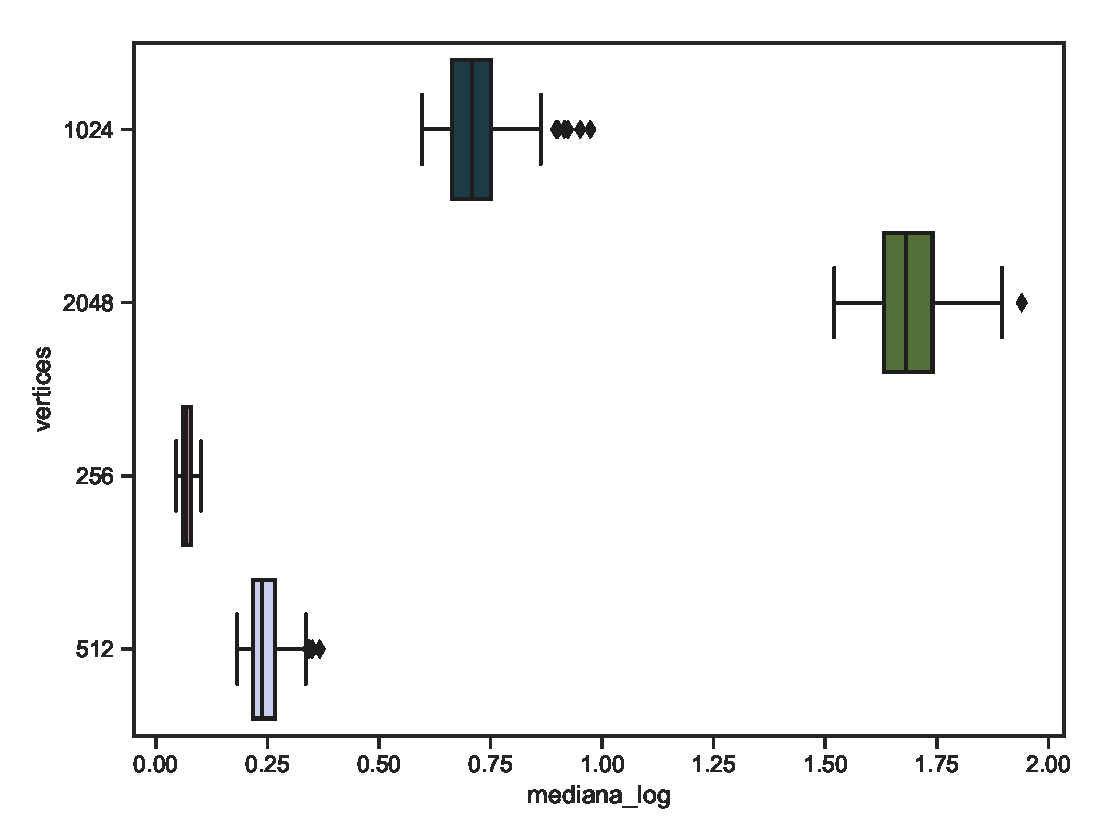
\includegraphics[scale=0.6]{boxplotvertices.eps}
\caption{Diagrama de caja y bigotes que relaciona los tiempos de ejecución con el número de vértices.}
\label{fig6}
\end{figure}
\end{center}
% Table generated by Excel2LaTeX from sheet 'Tukeyvertices'
\begin{table}[htbp]
  \centering
  \caption{Tukey, influencia del número de vértices en el tiempo de ejecución.}
    \begin{tabular}{rrrrrl}
    \toprule
    \multicolumn{1}{l}{\textit{\textbf{group1}}} & \multicolumn{1}{l}{\textit{\textbf{group2}}} & \multicolumn{1}{l}{\textit{\textbf{meandiff}}} & \multicolumn{1}{l}{\textit{\textbf{lower}}} & \multicolumn{1}{l}{\textit{\textbf{upper}}} & \textit{\textbf{reject}} \\
    \midrule
          &       &       &       &       &  \\
    1024  & 2048  & 0.97  & 0.9606 & 0.9794 & \textit{True} \\
          &       &       &       &       &  \\
    1024  & 256   & -0.6445 & -0.6539 & -0.6352 & \textit{True} \\
          &       &       &       &       &  \\
    1024  & 512   & -0.4689 & -0.4782 & -0.4595 & \textit{True} \\
          &       &       &       &       &  \\
    2048  & 256   & -1.6146 & -1.624 & -1.6052 & \textit{True} \\
          &       &       &       &       &  \\
    2048  & 512   & -1.4389 & -1.4483 & -1.4295 & \textit{True} \\
          &       &       &       &       &  \\
    256   & 512   & 0.1757 & 0.1663 & 0.1851 & \textit{True} \\
    \bottomrule
    \end{tabular}%
  \label{tab:t5}%
\end{table}%

En el cuadro \ref{tab:t5} se puede observar que en todos los casos se rechaza la hipótesis.En la figura \ref{fig7} de la página \pageref{fig7} muestra claramente este hecho.
\begin{center}
\begin{figure}[htbp]
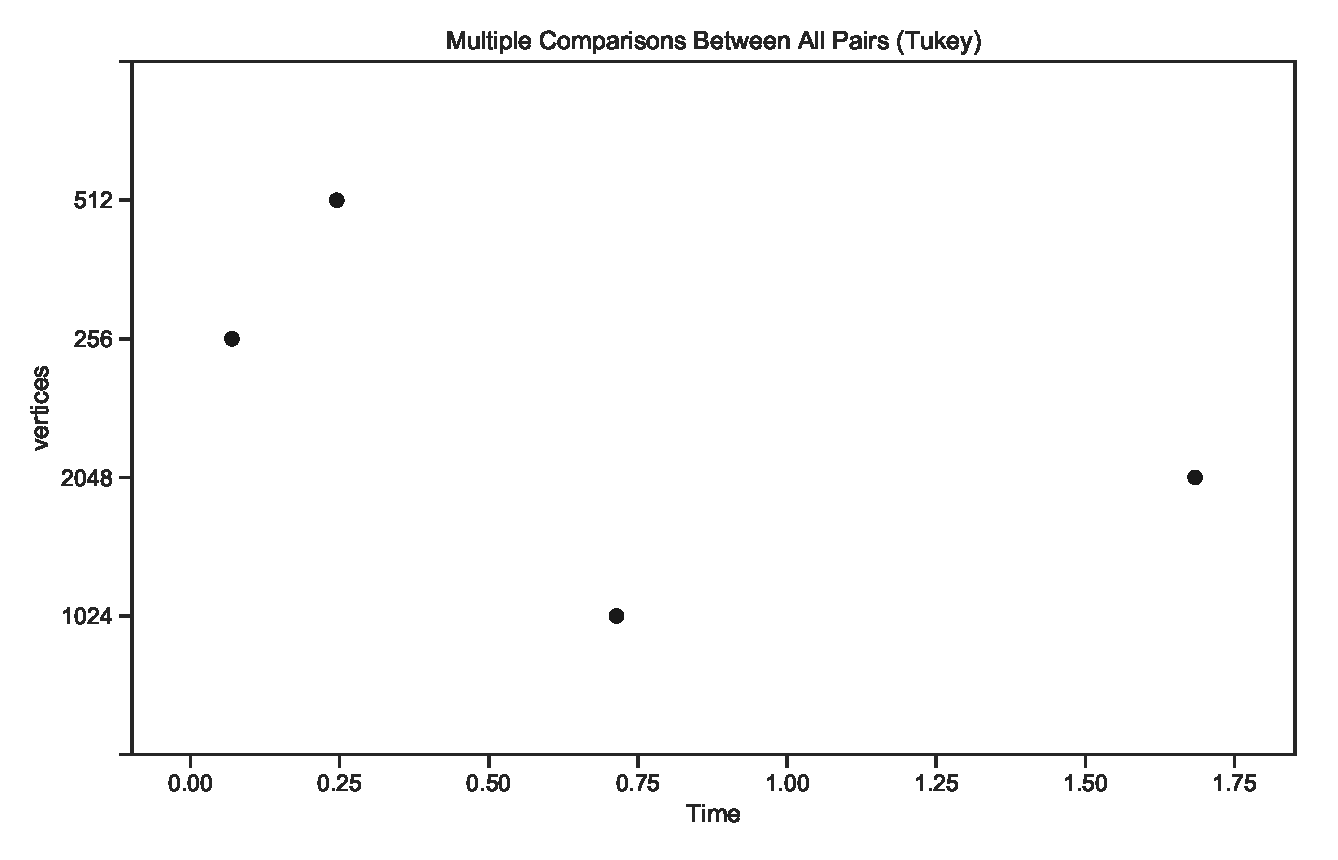
\includegraphics[scale=0.6]{simultaneoustukeyvertices.eps}
\caption{Diagrama simultaneo que relaciona los tiempos de ejecución con los grupos del factor número de vértices.}
\label{fig7}
\end{figure}
\end{center}
\subsubsection{Influencia de la densidad de los grafos en el tiempo de ejecución.}

En el caso del factor densidad se hizo una categorización por rangos para hacer cómoda la visualización de su relación con la variable dependiente estos rangos se obtuvieron a través de los contenedores que devolvió el histograma que se muestra en la figura \ref{fig3} de la página \pageref{fig3}.

\begin{center}
\begin{figure}[ht]
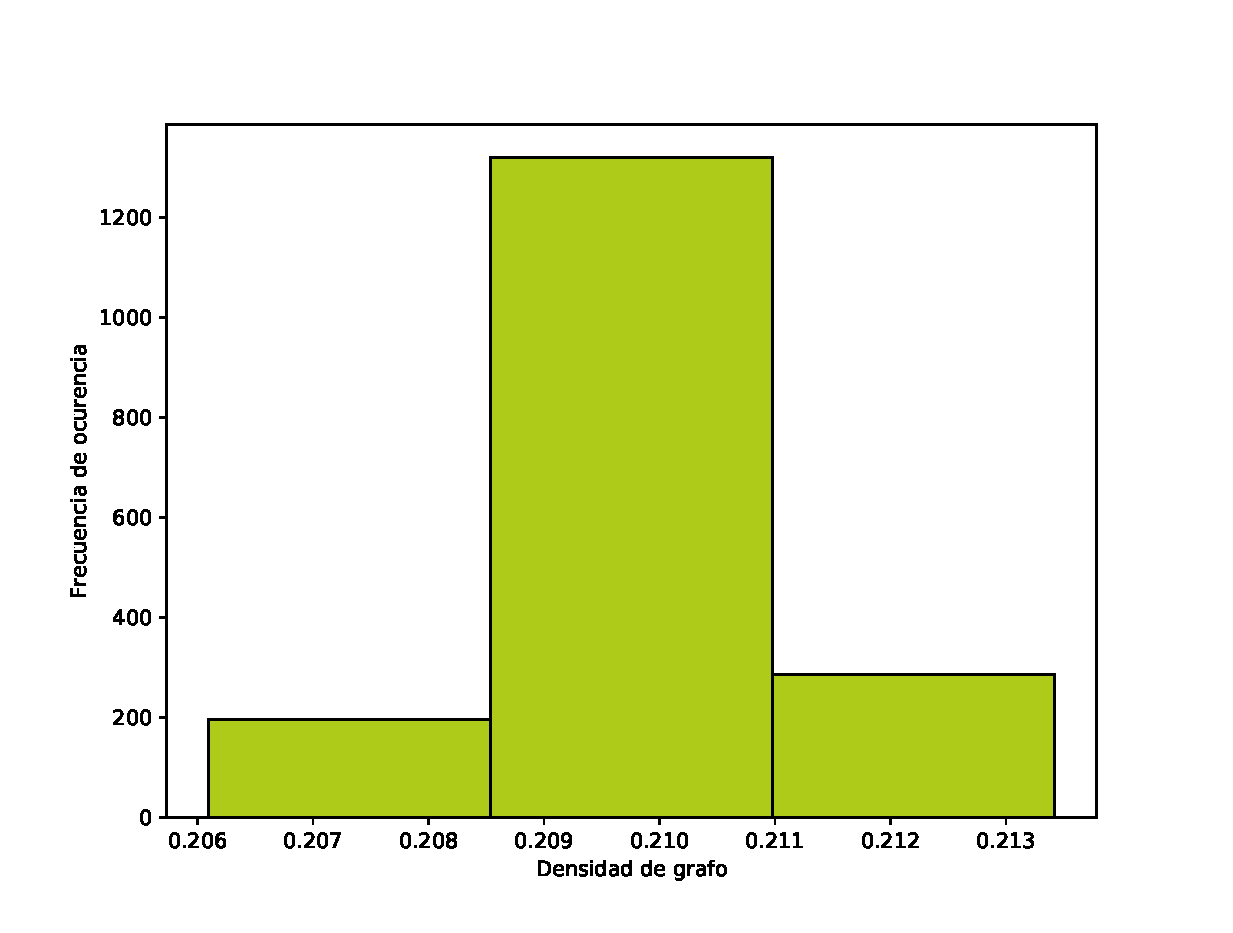
\includegraphics[scale=0.5]{boxplot.eps}
\caption{Histograma de densidad de los grafos.}
\label{fig3}
\end{figure}
\end{center}
El siguiente cuadro muestra el resultado de la aplicación del ANOVA.

% Table generated by Excel2LaTeX from sheet 'ANOVAdensidad'
\begin{table}[htbp]
  \centering
  \caption{ANOVA, influencia de la densidad de los grafos en el tiempo de ejecución.}
    \begin{tabular}{lrrrlll}
    \toprule
    \textbf{Factor} & \multicolumn{1}{l}{\textbf{SS}} & \multicolumn{1}{l}{\textbf{DF}} & \multicolumn{1}{l}{\textbf{MS}} & \textbf{F} & \textbf{p-unc} & \textbf{np2} \\
    \midrule
    densidad & 170.777 & 2     & 85.388 & \multicolumn{1}{r}{283.320} & \multicolumn{1}{r}{0.000} & \multicolumn{1}{r}{0.24} \\
    \textit{Within} & 541.589 & 1797  & 0.301 & -     & -     & - \\
    \bottomrule
    \end{tabular}%
  \label{tab:t6}%
\end{table}%
En el cuadro \ref{tab:t6} se muestra que como en elcuadro \ref{tab:t4} existen grandes diferencia entre las medianas de los grupos de factores ya que el $p-unc$ es menor que $0.05$ por lo que se se rechaza la hipótesis de que la densidad de los grafos no influye en el \textit{tiempo de ejecución}. Esto se puede observar en la figura \ref{fig8} de la página \pageref{fig8}. Por tal motivo se realiza la prueva de Tukey mostrara las diferencias entre las medianas de los factores, lo que se evidencia en el cuadro \ref{tab:t6} de la página \pageref{tab:t6}. 
\begin{center}
\begin{figure}[htbp]
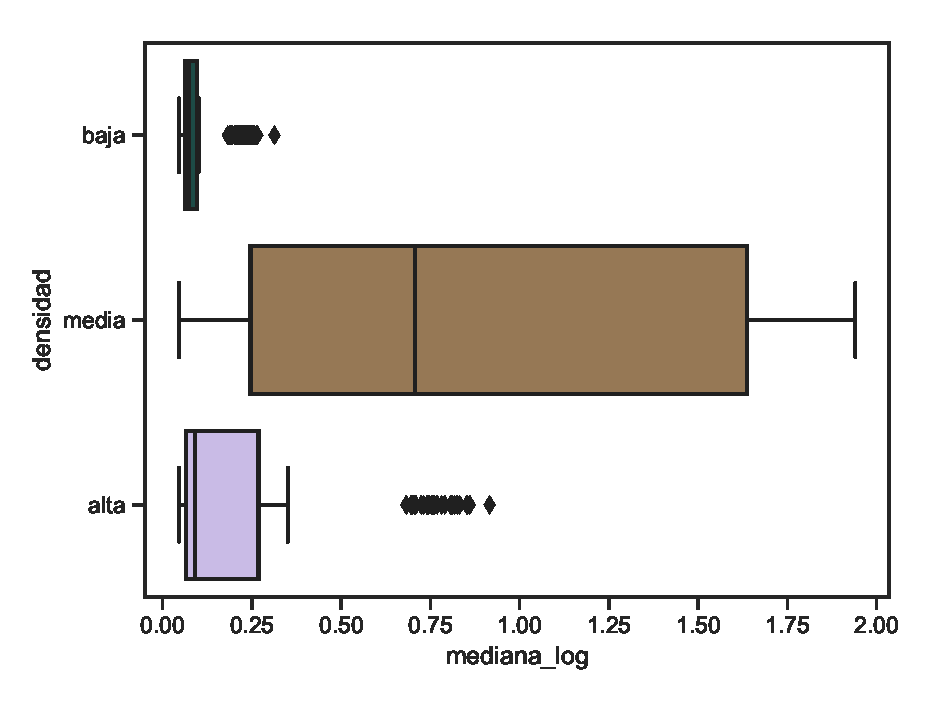
\includegraphics[scale=0.6]{boxplotdensidad.eps}
\caption{Diagrama de caja y bigotes que relaciona los tiempos de ejecución con la densidad de los grafos.}
\label{fig8}
\end{figure}
\end{center}

% Table generated by Excel2LaTeX from sheet 'Tukeydensidad'
\begin{table}[htbp]
  \centering
  \caption{Tukey,influencia de la densidad de los grafos en el tiempo de ejecución.}
    \begin{tabular}{llrrrl}
    \toprule
    \textit{\textbf{group1}} & \textit{\textbf{group2}} & \multicolumn{1}{l}{\textit{\textbf{meandiff}}} & \multicolumn{1}{l}{\textit{\textbf{lower}}} & \multicolumn{1}{l}{\textit{\textbf{upper}}} & \textit{\textbf{reject}} \\
    \midrule
    alta  & baja  & -0.1085 & -0.2281 & 0.0112 & \textit{False} \\
    alta  & media & 0.6497 & 0.5656 & 0.7338 & \textit{True} \\
    baja  & media & 0.7582 & 0.6594 & 0.8569 & \textit{True} \\
    \bottomrule
    \end{tabular}%
  \label{tab:t6}%
\end{table}%
En el cuadro \ref{tab:t6} se puede observar que en dos de los tres casos se rechaza la hipótesis y en el pareo de densidad alta y baja no existen diferencias stadísticas en cuanto a la mediana. En la figura \ref{fig9} de la página \pageref{fig9} muestra claramente este hecho.
\begin{center}
\begin{figure}[htbp]
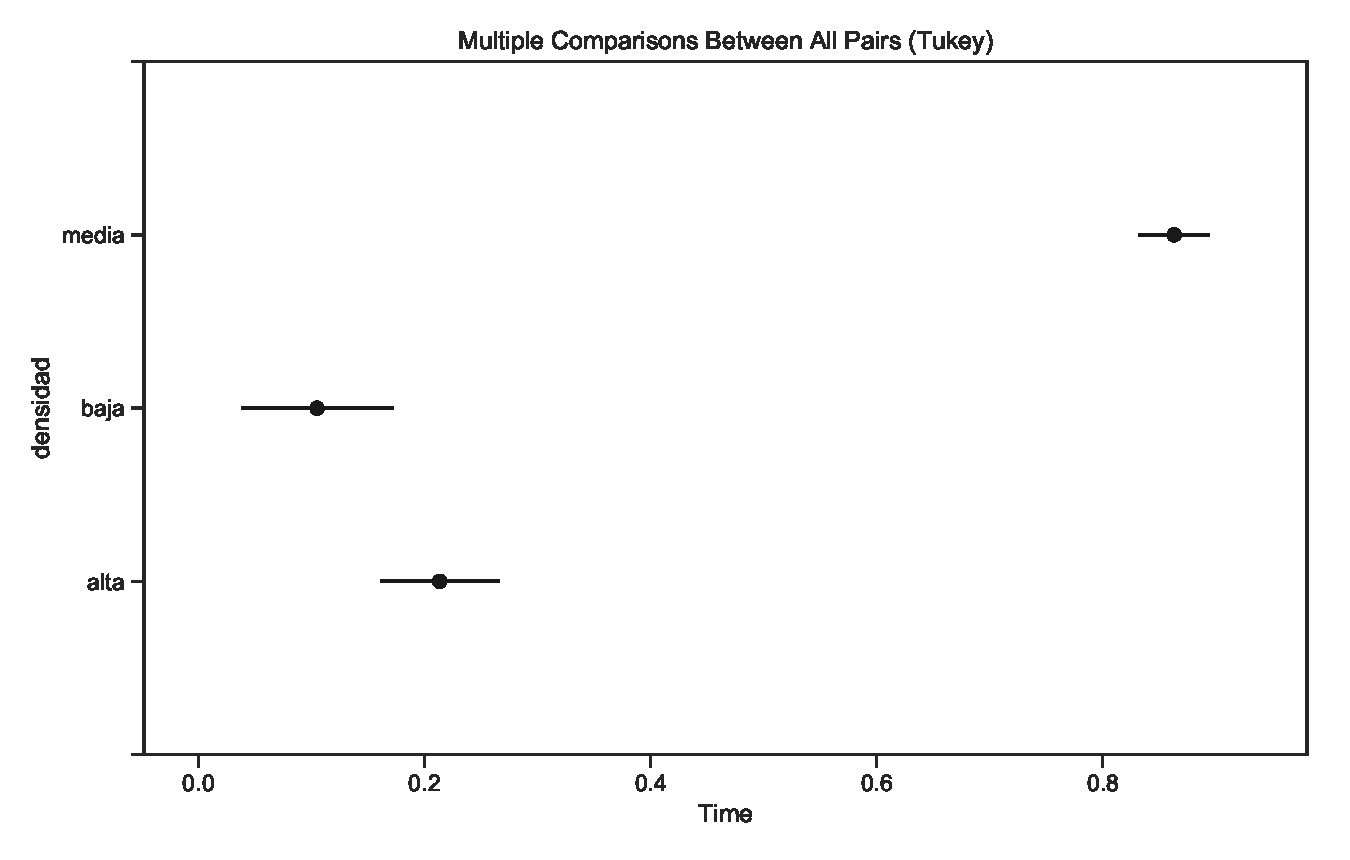
\includegraphics[scale=0.6]{simultaneoustukeydensidad.eps}
\caption{Diagrama simultaneo que relaciona los tiempos de ejecución con los grupos del factor densidad de los grafos.}
\label{fig9}
\end{figure}
\end{center}
\subsubsection{Influencia de los cuatro factores (algoritmo generador de grafo, algoritmo de flujo máximo, numero de vértices y densidad del grafo) en el tiempo de ejecución.}
Para analizar este caso se realizo ANOVA multifactorial dando como resultado el cuadro \ref{tab:t7} de la página \pageref{tab:t7}.

% Table generated by Excel2LaTeX from sheet 'modelo'
\begin{table}[htbp]
  \centering
  \caption{ANOVA multifactor, influencia de los cuatro factores en el tiempo de ejecución.}
    \begin{tabular}{lrrrr}
    \toprule
          & \multicolumn{1}{l}{\textbf{sum\_sq}} & \multicolumn{1}{l}{\textbf{df}} & \multicolumn{1}{l}{\textbf{F}} & \multicolumn{1}{l}{\textbf{\texttt{PR(>F)}}} \\
    \midrule
    generador\_grafo & 0.0291 & 2     & 33.0499 & 0.0000 \\
    algoritmo\_fm & -0.0001 & 2     & -0.1439 & 1.0000 \\
    vertices & 46.4767 & 3     & 35163.6974 & 0.0000 \\
    densidad & 0.0000 & 2     & 0.0000 & 0.9999 \\
    generador\_grafo:algoritmo\_fm & 0.0008 & 4     & 0.4714 & 0.7567 \\
    algoritmo\_fm:vertices & 0.0001 & 6     & 0.0248 & 0.8748 \\
    vertices:densidad & 0.0001 & 6     & 0.0425 & 0.9584 \\
    generador\_grafo:vertices & 0.0651 & 6     & 24.6313 & 0.0000 \\
    generador\_grafo:densidad & 0.0000 & 4     & 0.0181 & 0.8930 \\
    algoritmo\_fm:densidad & 0.0001 & 4     & 0.0425 & 0.9584 \\
    Residual & 0.7798 & 1770  &       &  \\
    \bottomrule
    \end{tabular}%
  \label{tab:t7}%
\end{table}%
En el cuadro \ref{tab:t7} se puede observar que los factores que más influyen en el tiempo de ejecución son el número de vértices y la densidad de los grafos, que además existe una relación entre el número de nodos y la densidad de los grafos. 

\newpage
\bibliographystyle{plain}
\bibliography{tarea4}

\end{document}
